\clearpage
\section{Code Triage and Transformations}
The second phase (shown in Fig.~\ref{fig:phase12}) includes code triage and a set of code transformations. 
Code triage relies on a ROSE-based tool interface to read in both source files and performance information of
the input application.
It then conducts various automated or user-directed analyses to identify
problematic code segments, such as loops. 
Finally, the identified code segments are extracted (also called outlined) into separated routines so they can be individually
optimized by empirical methods. 
%Since the analysis is on the AST or other graphs built
%using ROSE and uses the performance data stored as attributes, these analyses are
%expressed using traversals in ROSE.
\begin{figure}[htbp]
\vspace{5ex}
       \centering
               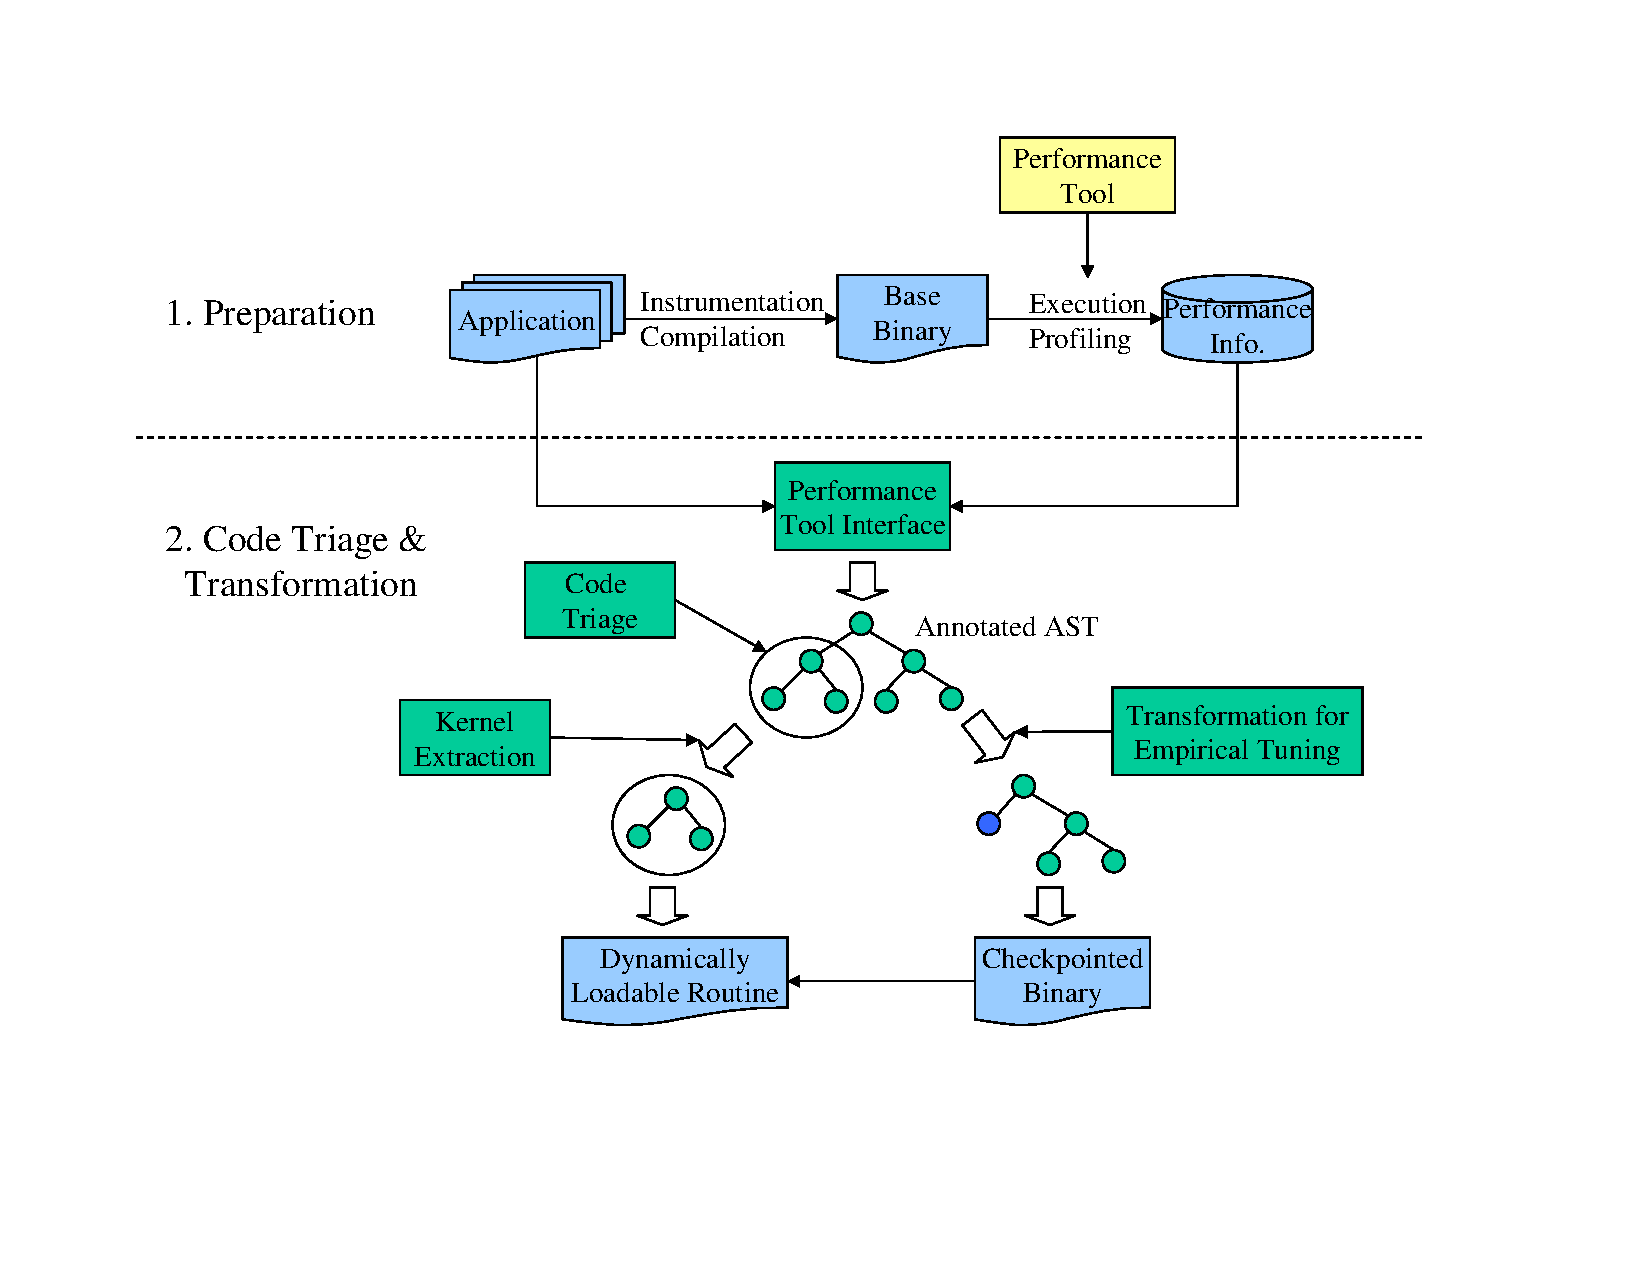
\includegraphics[width=1.2\textwidth]{phase12.pdf}
       \caption{Phase 1 and 2 of the autotuning system}
       \label{fig:phase12}
\end{figure}

%---------------------------------------------------
\subsection{Invoking Code Triage}
The source code for code triage is located in
\textit{rose/projects/autoTuning/autoTuning.C}. 
It already has initial implementation to call ROSE's tool interface,
conduct simple code triage, and finally extract kernels using ROSE's AST
outliner. 

With the input application and its performance result available, 
%a straightforward method is used to identify the most time-consuming
%statements in the code.  
%Loop nests containing those statements are reported as a
%tuning candidate, if the loop nests exist.
users can invoke the ROSE-based code triage by using the following command:

{\mySmallFontSize
\begin{verbatim}
autoTuning -c  jacobi.c -rose:hpct:prof jacobi-raw.xml \
-rose:autotuning:triage_threshold 0.8 -rose:outline:output_path "tests"
\end{verbatim}
}

The command above provides an input source file and its corresponding XML-format performance data generated by HPCToolkit.
It asks the code triage program to find the most time-consuming 
loops which account for just above 80\% of the total execution time. 
The identified loops will be automatically extracted to separated,
source files and saved into an output path named \textit{tests}.

Users can also enable code triage only without calling outlining. 
The performance data can come from GNU gprof. 
An example is given below:

%{\scriptsize
{\mySmallFontSize
\begin{verbatim}
# example command line to perform code triage only.
autoTuning  -c jacobi.c -rose:autotuning:triage_only -rose:gprof:linebyline jacobi.gprof.txt 

# the output is a list of abstract handles and 
# their corresponding execution time percentage
-----------------------------------------------------------------
The abstract handles for hot statements exceeding the threshold are:
Project<numbering,1>::SourceFile<name,/home/liao6/jacobi.c>::\
ExprStatement<position,193.9-194.76>
0.382
Project<numbering,1>::SourceFile<name,/home/liao6/jacobi.c>::\
ExprStatement<position,196.9-196.45>
0.3643
Project<numbering,1>::SourceFile<name,/home/liao6/jacobi.c>::\
ExprStatement<position,188.9-188.29>
0.11
-----------------------------------------------------------------
The abstract handles for enclosing loops for hot statements exceeding the
threshold are:
Project<numbering,1>::SourceFile<name,/home/liao6/jacobi.c>::\
ForStatement<position,190.5-198.7>
0.8189
\end{verbatim}
}

The above example command identifies a list of the most time-consuming statements and loops and reports them using abstract handles. 
The report will end once the sum of execution time of the statements or
loops reach or exceed a preset threshold (default is 75\% of the total execution time). 

We explain some details for the implementation of code triage and
autotuning-related transformations in the following subsections.
%----------------------------------------
\subsection{Tool Interface}
%A ROSE tool interface is required for understanding the performance results of each
%external performance tool. 
ROSE has a performance tool interface, called ROSE-HPCT,
in its distribution to accept performance results generated by external
performance tools .  
%Please follow the instructions from ROSE
%Tutorial's Chapter ROSE-HPCToolkit Interface to enable and use this module. 
Basically, it reads in the XML files generated from HPCToolkit and attaches performance metrics to
the ROSE AST representing the corresponding source code.
It can handle macro expansions during the metric match process.
When necessary, all performance metrics are also propagated from statement
levels to loop, function, and file levels. 
Similarly, it also accepts the line-by-line performance data generated by GNU
gprof.
%Currently, the ROSE-HPCToolKit interface is used to accept performance
%data generated by HPCToolkit and GNU gprof.
%The interface is used to annotate ROSE AST with performance metrics to
%facilitate building automated performance analysis tools. 
Detailed information about ROSE-HPCToolKit can be found in Chapter 44 of
the \htmladdnormallink{ROSE Tutorial}{http://www.rosecompiler.org/ROSE_Tutorial/ROSE-Tutorial.pdf}.
%We only give information relevant to autotuning below.

The code triage program uses the following code to invoke ROSE-HPCT.

{\mySmallFontSize
\begin{verbatim}
int main(int argc, char * argv[]) 
{
  vector<string> argvList (argv, argv+argc);
  // Read into the XML files
  RoseHPCT::ProgramTreeList_t profiles = RoseHPCT::loadHPCTProfiles (argvList);
  // Create the AST tree
  SgProject * project = frontend(argvList);
  //Attach metrics to AST , last parameter is for verbose
  RoseHPCT::attachMetrics(profiles, project,project->get_verbose()>0);
  //...
}
\end{verbatim}
}

%%----------------------------------------
%\subsection{Code Triage}
%A code triage module examines the AST annotated with
%performance metrics to locate problematic code portions (we call these code portions
%as autotuning targets).
%Currently, a straightforward top-down method is used to identify a hot spot
%in the code from the most time consuming file and then the loop nests containing such spot is reported as a
%tuning candidate, if the loop nests exist. The example code is shown below:
%\fixme{ROSE's AST merge could be used in the future to have a global view
%of AST merged from multiple source files.}
%
%{\mySmallFontSize
%\begin{verbatim}
% std::string hot_file = findHottestFile(fileMetrics);
% SgNode* hot_node=findHottestStatement(file, nodesWithMetrics);
% SgForStatement* target_loop= findTargetLoop(hot_node);
%
%\end{verbatim}
%}
%
%Code triage is also designed to suggest a set of potentially beneficial optimizations and
%their configuration ranges to improve the performance.
%\fixme{TODO need to implement this by compiler analysis. We manually 
% use the limited optimization choices, such as loop unrolling, by default for now.}
%
% DQ: Liao, what is the best entry point for me to write such a module/traversal.
% I think it would be good to have this in place before we release this document.
% I will be happy to write this part.

%----------------------------------------
\subsection{Kernel Extraction: Outlining}
Each of the identified tuning targets, often loops, will be extracted from the original code to
form separated functions (or routines). 
The ROSE AST outliner is invoked to generate such functions. 
%It replaces a block of consecutive statements with a function call to a newly generated
%function containing those statements. 
This kernel extraction step can be automatically invoked by the code triage
program or manually initiated by users via the outliner's command line
interface. 

The ROSE AST outliner handles multiple input languages, including C, C++ and
recently Fortran.  It also provides both command line and programming interfaces for users
to specify the targets to be outlined.  
Detailed information of using the ROSE outliner can be found in
Chapter 27 of the \htmladdnormallink{ROSE
Tutorial}{http://www.rosecompiler.org/ROSE_Tutorial/ROSE-Tutorial.pdf}.
You can also refer to a paper~\cite{LiaoEffective2009} for the algorithm we use to outline kernels. 
%More details of the ROSE AST outliner are
%available in the ROSE Tutorial's Chapter, Function Outlining using the AST Outliner.
For the code triage program, the programming interface of the Outliner is
used as below:

{\mySmallFontSize
\begin{verbatim}
  // recognize options for outliner
  Outliner::commandLineProcessing(argvList);
  ...
 SgForStatement* target_loop= findTargetLoop(hot_node);
 if (isOutlineable (target_loop))  
   outline(target_loop);
\end{verbatim}
}

The ROSE AST outliner accepts user options to further guide its internal
behavior. \lstinline{-rose:outline:parameter_wrapper } will wrap all
parameters of the outlined function into an array of pointers. 
\lstinline{-rose:outline:new_file} will separate the outlined function into
a new source file to facilitate external tools for further handling.
\lstinline{-rose:outline:use_dlopen} will transform the code to use
\lstinline{dlopen()} and \lstinline{dlsym()} to dynamically load the
outlined function from a library.

For the SMG2000 example, the most time-consuming loop is outlined and a call to it is used
to replace the loop in the original code. 
The loop is actually expanded from a macro
\lstinline{hypre_BoxLoop3For()}. 
ROSE is able to identify it after a bottom
up metrics propagation phase in ROSE-HPCT. 
%\fixme{Need to come up a way to automatically handle this, Should we
%do it within the outliner itself or before calling the outliner?})
The kernel extraction's result is shown in the following code listing:
\lstset{language={C},basicstyle=\scriptsize} 
\lstinputlisting{smg2000_outlined.fold.c}
\lstset{language={C},basicstyle=\small} 

%\fixme{TODO 
%   Also we should evaluate the overhead of this
%   step if the final result is an optimized function represented as a separate 
%   file (potentially disables some optimizations).  In the final assembly 
%   we could remove the dynamic linking, but the Makefile would have to be modified which
%   gets messy for an automated system.}

The ROSE outliner uses a variable cloning method to
avoid using pointer dereferencing within the outlined computation kernels. 
The method is based on usage of a variable that is passed by reference and
accessed
via pointer-dereferencing by classic outlining algorithms.
Such a variable is used either by value or by address within an outlining
target.
For the C language, using the variable by address occurs when the
address operator
is used with the variable (e.g. \lstinline{&X}).
C++ introduces one more way of using the variable by address:
associating the variable with a reference type
(\lstinline{TYPE & Y = X;} or using the variable as an argument for a
 function's parameter of a reference type).
If the variable is not used by its address,
a temporary clone variable of the same type (using \lstinline{TYPE clone;})
can be introduced to substitute its uses within the outlined function.
The value of a clone has to be
initialized properly (using \lstinline{clone = * parameter;})
before the clone participates in computation.
After the computation, the original variable must be set to the clone's
final value
(using \lstinline{*parameter = clone}).
By doing this, many pointer dereferences introduced by the classic
algorithm can be avoided.
\fixme{We are working on using liveness analysis to further eliminate unnecessary
value assignments.}

For easier interaction with other tools, the outlined function is separated
into a new source file, usually named after 
the function name.  
The ROSE outliner will recursively find and copy all dependent type declarations
into the new file to make it compilable.
For the SMG2000 example, a file named out\_1\_6755\_\_.orig.c 
is generated and it only contains the function body of \lstinline{OUT_1_6755__()}. 
This file will be transformed by a parameterized optimizer to a kernel
variant named OUT\_\_1\_\_6755\_\_.c and further compiled into a dynamically
loadable routine.

A sample makefile to generate the .so file is given below: 

{\mySmallFontSize
\begin{verbatim}
[liao@localhost smg2000] cat makefile-lib
lib:OUT__1__6755__.so
OUT__1__6755__.o:OUT__1__6755__.c
        gcc -c -fpic OUT__1__6755__.c
OUT__1__6755__.so:OUT__1__6755__.o
        gcc -shared -lc -o OUT__1__6755__.so OUT__1__6755__.o
clean:
        rm -rf OUT__1__6755__.so OUT__1__6755__.o
\end{verbatim}
}

%----------------------------------------
\subsection{Transformations for Autotuning}
The call site of the outlined function in the source code has to be further transformed to support empirical optimization. 
These transformations include:
\begin{itemize}
\item using \lstinline{dlopen()} to open a specified .so file containing
the outlined target and calling the function found in the file,
\item adding performance measuring code to time the call of the outlined target function.
\item transforming code to support checkpointing the execution right before
\lstinline{dlopen()} opening the library source file so multiple variants of the file can be used to test optimization choices empirically when the program is restarted multiple times.
\end{itemize}
%\fixme{TODO the code translations in this sub section are manually done
%now. We will start to
%implement them once the translation methods are agreed on by partners.}
%----------------------------------------
\subsubsection{Calling a Function Found in a .so File}
As mentioned earlier, the outlined function containing the target kernel is
stored in a separated source file, which will be transformed into a kernel variant
and then compiled to a dynamically loadable library. 
The original source code has to be transformed to open the library file,
find the outlined function, and finally call it using the right
parameters. An example of the resulting transformation on the function containing the
outlined loop is given below:
\lstset{language={C}, basicstyle=\scriptsize}
\lstinputlisting{smg2000_dlopen.c}

\subsubsection{Timing the Call}
The call to the outlining target kernel should be timed to get the
evaluation results during the empirical optimization. 
We instrument the call as follows to get the performance evaluation of a
kernel variant. 
More accurate and less intrusive methods based on hardware
counters can also be used in the future. 

{\mySmallFontSize
\begin{verbatim}
//save timing information into a temporary file

remove("/tmp/peri.result");
time1=time_stamp();
// parameter wrapping statements are omitted here
(*OUT__1__6755__)(__out_argv1__1527__);

time2=time_stamp();
FILE* pfile;
pfile=fopen("/tmp/peri.result","a+");
if (pfile != NULL)
{
  fprintf(pfile,"%f\n",time2-time1);
  fclose(pfile);
}
else
  printf("Fatal error: Cannot open /tmp/peri.result!\n");

\end{verbatim}
}

%----------------------------------------
\subsubsection{Checkpointing and Restarting}
In order to efficiently evaluate hundreds or even thousands of kernel
variants, we use a checkpointing and restarting method to measure the time
spent on calling the kernel without unnecessarily repeating the execution
before and after calling the kernel.  This allows the full context (state) 
of the application to be used in the evaluation of the kernel performance.
\fixme{need to discuss the drawbacks, e.g. missing cache warmup; and how that
might be addressed in the future by pushing back the checkpoint start and 
transformations to the checkpointed program (later).}

The Berkeley Lab Checkpoint/Restart (BLCR) library~\cite{blcrWeb} was selected for its
programmability, portability and robustness. 
BLCR is designed to support asynchronous checkpointing, which means a running process
is notified by another process to be checkpointed first, but the exact checkpointing
action happens on an indeterministic point later on. 
This default behavior is not desired for our purpose since we want an
accurate source position to do the checkpointing. 
Fortunately, BLCR's library does provide some internal functions to help
us initiate synchronous (immediate) checkpointing, though not well documented. 
After some trial and error rounds, we use the following code transformation
to have a synchronous checkpointing using the blcr-0.8.2 release.
The idea is to have a running program to notify itself to initiate a checkpointing. 
The program is then blocked until the request is served. 

To support BLCR, we have transformed the original source code in two locations.
% Two places in the source files have to be changed. 
The first location is the file where the main() function exists. We add the necessary
header files and initialization codes for using BLCR.  For example:
\lstset{language={C}, basicstyle=\scriptsize}
\lstinputlisting{smg2000_checkpoint.c}
% \lstset{language={C}, basicstyle=\small}

The second place is the actual source line to initiate the checkpointing. 
A checkpoint argument structure is filled out first to customize the
behavior we want, including the scope, target, memory dump file,
consequence, and so on. A blocking phase is put right after
\lstinline{cr_request_checkpoint()} to have an immediate checkpointing.
Our goal is to stop the executable right before opening the .so file so
a different kernel variant can be compiled into the .so file each time. 
The execution will be restarted multiple times so multiple variants can 
be evaluated this way. 

\lstset{language={C}, basicstyle=\scriptsize}
\lstinputlisting{smg2000_checkpoint2.c}
% \lstset{language={C}, basicstyle=\small}

Only these minimum transformations are needed to build the target application to support
BLCR. We choose the static linking method to support BLCR as follows.
The BLCR library is linked with the final executable. 

{\mySmallFontSize
\begin{verbatim}
smg2000: smg2000.o
        @echo  "Linking" \$@ "... "
        \${CC} -o smg2000 smg2000.o \${LFLAGS} -lcr
\end{verbatim}
}

The checkpointed binary has to be executed once to generate a memory dump
file (process image), which can then be reused multiple times to restart the execution 
immediately before the line where \lstinline{dlopen()} is invoked to evaluate multiple
variants of the optimization target kernel.

{\mySmallFontSize
\begin{verbatim}
[liao@localhost test] ./smg2000 -n 120 120 120 -d 3
current process ID is 6028
Running with these driver parameters:
  (nx, ny, nz)    = (120, 120, 120)
  (Px, Py, Pz)    = (1, 1, 1)
  (bx, by, bz)    = (1, 1, 1)
  (cx, cy, cz)    = (1.000000, 1.000000, 1.000000)
  (n_pre, n_post) = (1, 1)
  dim             = 3
  solver ID       = 0
=============================================
Struct Interface:
=============================================
Struct Interface:
  wall clock time = 0.550000 seconds
  cpu clock time  = 0.540000 seconds
Checkpoiting: stopping here ..
Killed
\end{verbatim}
}

A context dump file named dump.yy will be generated by BLCR as the
checkpointing result. This dump file will be used to restart the execution using
the command: \lstinline{cr_restart dump.yy}.
